
\chapter{Fundamentos y propiedades de los fluidos.}
	\section{Hipótesis de medio continuo.}
Un fluido se caracteriza por un volumen (V) y una longitud característica (L) donde:

\[L \approx V^{\dfrac{1}{3}}\]

%\begin{figure}[H]
%	\centering
%	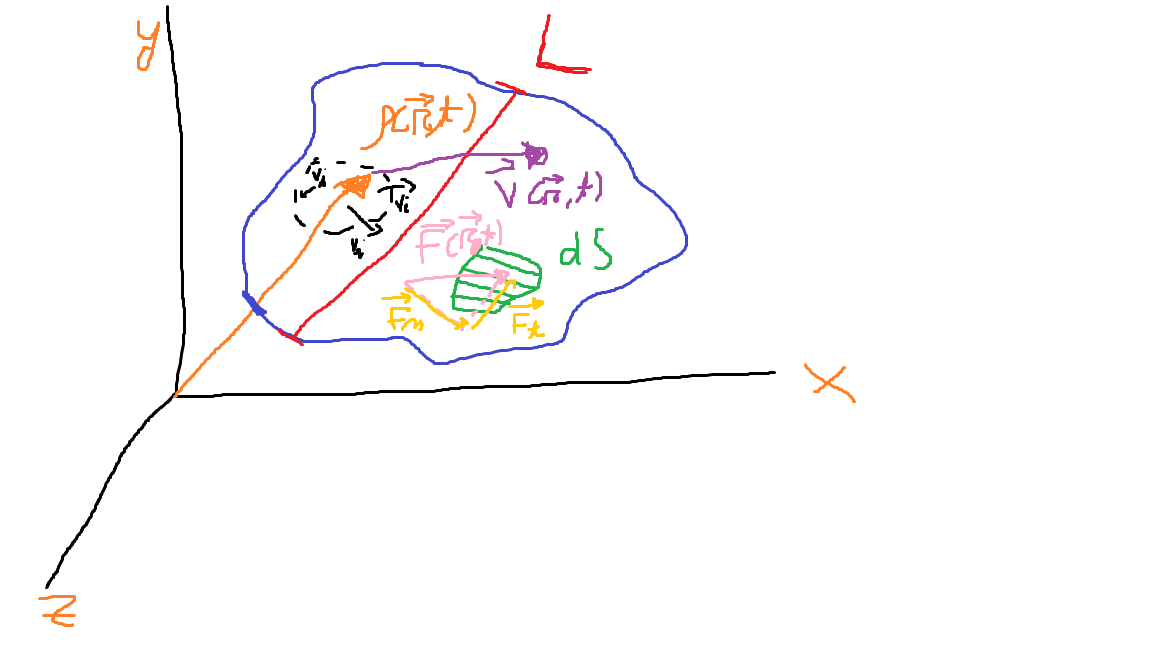
\includegraphics[width=0.5\linewidth]{imagenesTema1/caracteristicasFluido}
%	
%	\caption{Magnitudes fundamentales de un fluido.}
%	\label{fig:caracteristicasfluido}
%\end{figure}

\begin{figure}[H]
	\centering
		\begin{circuitikz}
			\tikzstyle{every node}=[font=\normalsize]
			\draw [-latex] (7.5,14.75) -- (7.5,19.75)node[pos=1,above]{y};
			\node [color=orange] at (11.25,17.85) {$\rho(\vec{r},t)$};
			\draw [-latex] (7.5,14.75) -- (12.5,14.75)node[pos=1,right]{x};
			\draw [-latex] (7.5,14.75) -- (5,12.25)node[pos=1,left]{z};
			\draw [, dashed] (10.5,17.75) ellipse (1.5cm and 0.2cm);
			\draw [short] (9,17.75) .. controls (9,18.25) and (8.75,18.25) .. (9,19);
			\draw [short] (9,19) .. controls (9.75,20.5) and (10.75,20) .. (11.25,19.75);
			\draw [short] (11.25,19.75) .. controls (12.25,19.25) and (11.75,18.75) .. (12,17.75);
			\draw [short] (12,17.75) .. controls (12,17) and (12,17) .. (11.5,16.5);
			\draw [short] (11.5,16.5) .. controls (11,16.25) and (11,16) .. (9.75,16.25);
			\draw [short] (9.75,16.25) -- (9.25,16.5);
			\draw [short] (9.25,16.5) .. controls (8.75,17) and (9.25,17.25) .. (9,17.75);
			\node [font=\normalsize] at (9,19.5) {V};
			\draw [ fill={rgb,255:red,168; green,255; blue,168} ] (10,19) circle (0.5cm);
			\draw [, dashed] (10,19) ellipse (0.5cm and 0.1cm);
			\node [font=\normalsize] at (10.75,19.25) {dV};
			\draw [ color={rgb,255:red,255; green,0; blue,0}, latex-latex] (11.75,19.25) -- (9.25,16.5)node[pos=0.8,sloped,above]{L};
			\draw [ fill={rgb,255:red,168; green,255; blue,168} ] (11,16.75) ellipse (0.5cm and 0.25cm);
			\node [font=\normalsize] at (11.5,17.25) {dS};
			\draw [ color={rgb,255:red,255; green,128; blue,255}, -latex] (10.25,16.75) -- (11,16.75)node[pos=0.5,above]{$\vec{F}(\vec{r},t)$};
			\draw [ color={rgb,255:red,255; green,0; blue,128}, -latex] (10.25,16.75) -- (10.75,16.25)node[pos=0.2,below]{$\vec{F}_m$};
			\draw [ color={rgb,255:red,255; green,0; blue,128}, -latex] (10.75,16.25) -- (11,16.75)node[pos=0.5,right]{$\vec{F}_t$};
			\draw [ color={rgb,255:red,128; green,0; blue,255}, -latex] (10,19) -- (12.5,19)node[pos=1,right]{$\vec{v}(\vec{r},t)$};
			\draw [-latex] (10,19) -- (9.75,19.75)node[pos=1,right]{$\vec{v}_i$};
			\draw [-latex] (10,19) -- (9.25,18.5)node[pos=0.95,above]{$\vec{v}_i$};
			\draw [-latex] (10,19) -- (10.75,18.5)node[pos=1,above]{$\vec{v}_i$};
			\draw [-latex] (7.5,14.75) -- (10,19)node[pos=0.5,sloped,above]{$\vec{r}(t)$};
		\end{circuitikz}
	\caption{Magnitudes fundamentales de un fluido.}
	\label{fig:caracteristicasfluido}
\end{figure}

Como el tamaño de una molécula es de $d_0 \approx 10^{-11} \ a \ 10^{-10}\,m$, la longitud característica debe ser mucho mayor que $d_0$ ($L>\!>d_0$) para así comprender el número suficiente de moléculas y poder estudiar la mecánica de fluidos de manera macroscópica.\\

Además, la longitud debe ser suficiente para que exista equilibrio termodinámico local y así poder aplicar las ecuaciones de estado:

\begin{itemize}
	\item Camino libre medio ($\lambda$) de interacción por choque entre moléculas.
	\begin{itemize}
		\item En líquidos: $\lambda \approx d_o$
		\item En gases: $\lambda >\!> d_o$
	\end{itemize}
	\[L >\!> \lambda\]
\end{itemize}

%\begin{figure}[H]
%	\centering
%	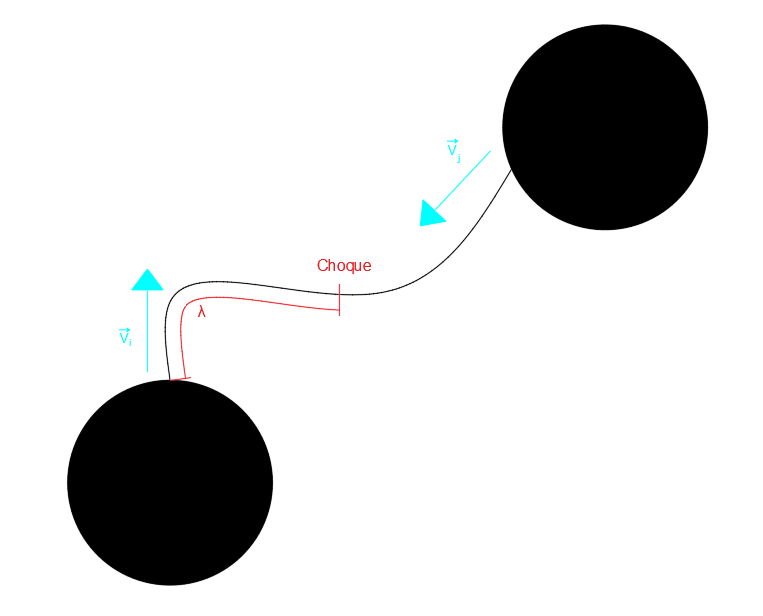
\includegraphics[width=0.35\linewidth]{imagenesTema1/caminoLibreMedio}
%	\caption{Camino libre medio.}
%	\label{fig:caminolibremedio}
%\end{figure}

\begin{figure}[H]
	\centering
		\begin{circuitikz}
			\tikzstyle{every node}=[font=\normalsize]
			\draw [ fill={rgb,255:red,0; green,128; blue,255} ] (3.75,19.75) circle (0.5cm);
			\draw [ fill={rgb,255:red,0; green,128; blue,255} ] (9,19.75) circle (0.5cm);
			\draw [short] (8.5,19.75) .. controls (4.5,18) and (7.75,22) .. (4.25,19.75);
			\draw [ color={rgb,255:red,0; green,128; blue,255}, -latex] (3.75,20.25) -- (3.75,21.5)node[pos=1,above]{$\vec v_1$};
			\draw [ color={rgb,255:red,0; green,128; blue,255}, -latex] (8.5,19.75) -- (7.5,20.5)node[pos=1,above]{$\vec v_2$};
			\draw [color={rgb,255:red,255; green,0; blue,0}](6.25,19.75) to[short, -*] (6.25,19.75);
			\node [font=\normalsize, color={rgb,255:red,255; green,0; blue,0}] at (5.5,19.75) {Choque};
			\draw [ color={rgb,255:red,255; green,0; blue,0}, short] (6.25,19.75) -- (6.75,19.75);
			\draw [ color={rgb,255:red,255; green,0; blue,0}, short] (4.25,20.25) -- (4.25,19.75);
			\draw [ color={rgb,255:red,255; green,0; blue,0}, latex-latex] (4.25,20) .. controls (5.25,20.75) and (6.5,21.25) .. (6.5,19.75)node[pos=0.5,above]{$\lambda$};
		\end{circuitikz}
	\caption{Camino libre medio.}
	\label{fig:caminolibremedio}
\end{figure}

En este fluido es necesario poder medir:
\begin{enumerate}
	\item \underline{\textbf{Densidad}}: el diferencial de volumen debe ser una muestra significativa a nivel estadístico.
	
	\[\rho(\vec{r},t)=\lim_{{V \to 0}} \frac{\Delta m}{\Delta V}=\frac{dm}{dV} \ \left[{\frac{kg}{m^3}}\right]\] 
	
	
	\begin{itemize}
		\item El fluido es un gas si: $\rho \neq cte \Rightarrow \rho=f(\vec{r},t)$
		\item El fluido es un líquido si: $\rho = cte \Rightarrow \rho=f(t)$
	\end{itemize}
	
	Si la función depende del tiempo, se dice que está en forma paramétrica.
	
	\begin{itemize}
		\item Peso específico
		\[\gamma=\rho g  \Rightarrow g: \text{campo gravitatorio} \left[{\frac{m}{s^2}}\right]\]
		\item Densidad relativa
		\[\rho_{rel}=\frac{\rho}{\rho_{ref}}\]
		
		\begin{itemize}
			\item Líquidos: $\rho_{ref}=\rho_{agua}\approx 10^3 \frac{kg}{m^3}$
				\item Gases: $\rho_{ref}=\rho_{aire_{CN}}\approx 1 \frac{kg}{m^3}$
		\end{itemize}
	\end{itemize}
		
	\item \underline{\textbf{Velocidad}}:
		\[\vec{v}(\vec{r},t)=\lim_{{\Delta V \to 0}} \frac{\sum_i m_i \vec{v_i}}{\sum_i m_i} \left[{\frac{m}{s}}\right]\]
	\item \underline{\textbf{Presión}}: Es una magnitud absoluta (siempre mayor que 0):
	
	\[P=\frac{d(\vec{F}\cdot\vec{n})}{dS} =\frac{d{F_n}}{dS} [Pa]\]
	\[1\,bar = 10^5\,Pa\]
	\[1\,atm = 101325\,Pa\]
	\[1\,mmHg =\rho_{Hg}\cdot g\cdot h=132.32\,Pa\]
	\[1\,mca\text{ (metros de columna de agua)} = \rho_{H_2O}\cdot g\cdot h=9.8\cdot 10^3\,Pa\]
	\begin{itemize}
		\item Presión manométrica ($P_{man}$): Se mide normalmente con un manómetro diferencial:
		
		\[P_{man} = P - P_{atm} \Rightarrow P>P_{atm}\]
		\item Presión vacuométrica ($P_{vac}$): Se mide normalmente con un vacuómetro.
		
		\[P_{vac}= P_{atm}-P \Rightarrow P<P_{atm}\]
		
		\item Presión de vapor ($P_v$): Se refiere al equilibrio de fase líquido-gas. Si la presión es menor que la presión de vapor \textbf{cavita}.
		\item Cavitación: Generación de burbujas en el líquido por estar por debajo de la presión de vapor que posteriormente al subir la presión explotan con violencia. 
	\end{itemize}
	
\end{enumerate}

\section{Ecuaciones equilibrio termodinámico local.}
En un gas ideal, si las condiciones son subsónicas se cumple que:
\[\frac{P}{\rho}=R_gT \Rightarrow R_g\cdot\frac{R}{mmr} \Rightarrow R ={8.314} \frac{J}{mol\cdot K}\]

El fluido está en condiciones subsónicas si:
\[\left| \vec{v}(\vec{r},t) \right|<a=\sqrt {\left. \frac{\partial P}{\partial \rho} \right|}_{S=cte}\]

\begin{itemize}
	\item Ecuación isoentrópica: Procesos rápidos.
	\[PV^\alpha=cte\]
	\item Ecuación isoterma: Procesos lentos.
	\[PV=cte\]
\end{itemize}
\section{Fuerzas y respuestas en sólidos y fluidos}
\begin{enumerate}
	\item \underline{\textbf{Fuerzas en un fluido}}:
	\[F=f(\Delta \dot{x})=C\dot{x} \Rightarrow C: \text{constante de amortiguamiento}\]
	
	\item \underline{\textbf{Tensión tangencial o de cizalladura}}($\tau$):
	\[\tau=\lim_{{S \to 0}} \frac{\Delta F_t}{\Delta S}=\frac{dF_t}{dS}\]
	\item \underline{\textbf{Viscosidad}}($\mu$):
	En fluidos newtonianos la viscosidad es relativamente constante: 
	\[\mu=f(t) [Pa \cdot s]\]
	\[\tau =\mu \dot{\varepsilon} = \mu \frac{\Delta v_n}{\Delta l_n} \Rightarrow \dot{\varepsilon}\ \text{es la velocidad de deformación} [s^{-1}]\]
%\begin{figure}[H]
%	\centering
%	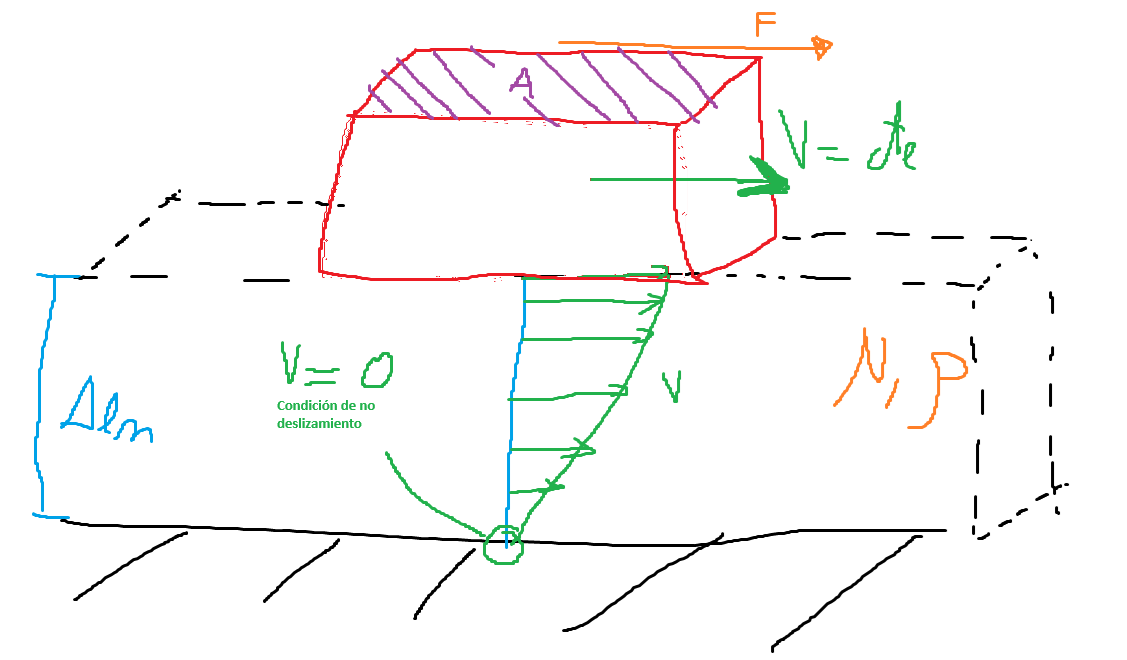
\includegraphics[width=0.7\linewidth]{imagenesTema1/viscosidad}
%	\caption{Cálculo de viscosidad.}
%	\label{fig:viscosidad}
%\end{figure}

\begin{figure}[H]
	\centering
		\begin{circuitikz}[scale = 0.8]
			\tikzstyle{every node}=[font=\normalsize]
			\draw [ color={rgb,255:red,255; green,0; blue,0}, short] (3,15.75) -- (3,14.25);
			\draw [ color={rgb,255:red,255; green,0; blue,0}, short] (3,14.25) -- (6,14.25);
			\draw [ color={rgb,255:red,255; green,0; blue,0}, short] (6,14.25) -- (6,15.75);
			\draw [ color={rgb,255:red,255; green,0; blue,0}, short] (6,15.75) -- (3,15.75);
			\draw [ color={rgb,255:red,255; green,0; blue,0}, short] (6,14.25) -- (6.5,14.75);
			\draw [ color={rgb,255:red,255; green,0; blue,0}, short] (6.5,14.75) -- (6.75,15);
			\draw [ color={rgb,255:red,255; green,0; blue,0}, short] (6.75,15) -- (6.75,16.5);
			\draw [ color={rgb,255:red,255; green,0; blue,0}, short] (6.75,16.5) -- (6,15.75);
			\draw [ color={rgb,255:red,255; green,0; blue,0}, short] (3,15.75) -- (3.75,16.5);
			\draw [ color={rgb,255:red,255; green,0; blue,0}, short] (3.75,16.5) -- (6.75,16.5);
			\node [font=\normalsize, color={rgb,255:red,255; green,0; blue,0}] at (4.75,16.125) {A};
			\draw [ color={rgb,255:red,255; green,128; blue,0}, -latex] (1,15) -- (3,15)node[pos=0.5,above]{$\vec{F}$};
			\draw [ color={rgb,255:red,0; green,128; blue,0}, -latex] (6.5,15.25) -- (8.5,15.25)node[pos=0.5,above]{$\vec{v}=cte$};
			\draw [short] (1.25,11) -- (8.75,11);
			\draw [short] (4,14.25) -- (4,11);
			\draw [ color={rgb,255:red,0; green,128; blue,0}, short] (4,11) -- (5.6,14.25)node[pos=0.5,right]{$\vec{v}(\Delta l)$};
			\draw [ color={rgb,255:red,0; green,128; blue,0}, -latex] (4,14) -- (5.5,14);
			\draw [ color={rgb,255:red,0; green,128; blue,0}, -latex] (4,13.5) -- (5.25,13.5);
			\draw [ color={rgb,255:red,0; green,128; blue,0}, -latex] (4,13) -- (5,13);
			\draw [ color={rgb,255:red,0; green,128; blue,0}, -latex] (4,12.5) -- (4.75,12.5);
			\draw [ color={rgb,255:red,0; green,128; blue,0}, -latex] (4,12) -- (4.5,12);
			\draw [ color={rgb,255:red,0; green,128; blue,0}, -latex] (4,11.5) -- (4.25,11.5);
			\draw [dashed] (6,14.25) -- (8.75,14.25);
			\draw [dashed] (6.75,15) -- (9,15);
			\draw [dashed] (3,14.25) -- (1.25,14.25);
			\node [font=\normalsize, color={rgb,255:red,255; green,128; blue,0}] at (8,13.5) {$\mu,$ $\rho$};
			\node [font=\normalsize] at (5.75,12.25) {};
			\node [font=\normalsize, color={rgb,255:red,255; green,0; blue,255}] at (3.25,11.25) {$v=0$};
			\draw [ color={rgb,255:red,255; green,0; blue,255} ] (4,11) circle (0.25cm);
			\draw [ color={rgb,255:red,0; green,128; blue,255}, latex-latex] (1.5,14.25) -- (1.5,11)node[pos=0.5,left]{$\Delta l_n$};
			\draw [short] (1.75,11) -- (1.25,10.5);
			\draw [short] (2.5,11) -- (2,10.5);
			\draw [short] (3.25,11) -- (2.75,10.5);
			\draw [short] (4,11) -- (3.5,10.5);
			\draw [short] (4.75,11) -- (4.25,10.5);
			\draw [short] (5.5,11) -- (5,10.5);
			\draw [short] (6.25,11) -- (5.75,10.5);
			\draw [short] (7,11) -- (6.5,10.5);
			\draw [short] (7.75,11) -- (7.25,10.5);
			\draw [short] (8.5,11) -- (8,10.5);
		\end{circuitikz}
	
	\caption{Cálculo de viscosidad.}
	\label{fig:viscosidad}
\end{figure}

\[\tau =\frac{F}{A}=\mu \frac{\Delta v_n}{\Delta l_n} =\mu \frac{v - 0}{l_n}= \mu \frac{v}{l_n}\]
	 
	 En fluidos no newtonianos la viscosidad no es constante:
	 
	 \begin{center}
	 	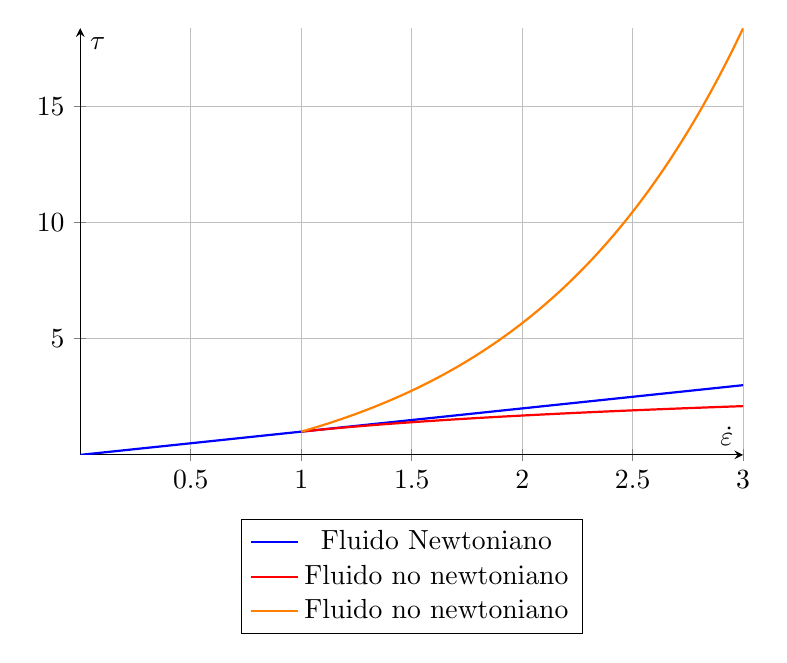
\begin{tikzpicture}
	 		\centering
	 		\begin{axis}[
	 			domain=0:3,
	 			samples=100,
	 			height=7cm,
	 			width=10cm,
	 			title={},
	 			ylabel=$\boldsymbol\tau$,
	 			xlabel=$\dot{\boldsymbol\varepsilon}$,
	 			grid=major,
	 			axis lines=center,
	 			legend style={at={(0.5,-0.15)}, anchor=north},
	 			]
	 			\addplot[blue, thick] {x};
	 			\legend{Fluido Newtoniano}
	 			
	 			\addplot[red, thick, domain=1:3] {ln(x)+1};
	 			\addlegendentry{Fluido no newtoniano}
	 			
	 			\addplot[orange, thick, domain=1:3] {e^x-e^1+1};
	 			\addlegendentry{Fluido no newtoniano}
	 		\end{axis}
	 	\end{tikzpicture}
	 \end{center}
	 
	 Viscosidades típicas:
	 \[\mu_{H_2O}=10^{-3} Pa \cdot s = 1\,cP \Leftarrow \text{centipoise}\]
	\item \underline{\textbf{Viscosidad cinemática}}:
	\[\nu = \frac{\mu}{\rho} \left[\frac{m^2}{s}\right] \Rightarrow 1\,csk = 10^{-6}\left[\frac{m^2}{s}\right] \Leftarrow \text{centistoke}\]
	
	\item \underline{\textbf{Interfases}}: 
	\begin{itemize}
		\item Vaso grande: Existe intercambio de moléculas en la interfase pero las presiones se equilibran.
		 %\begin{figure}[H]
		 %	\centering
		 %	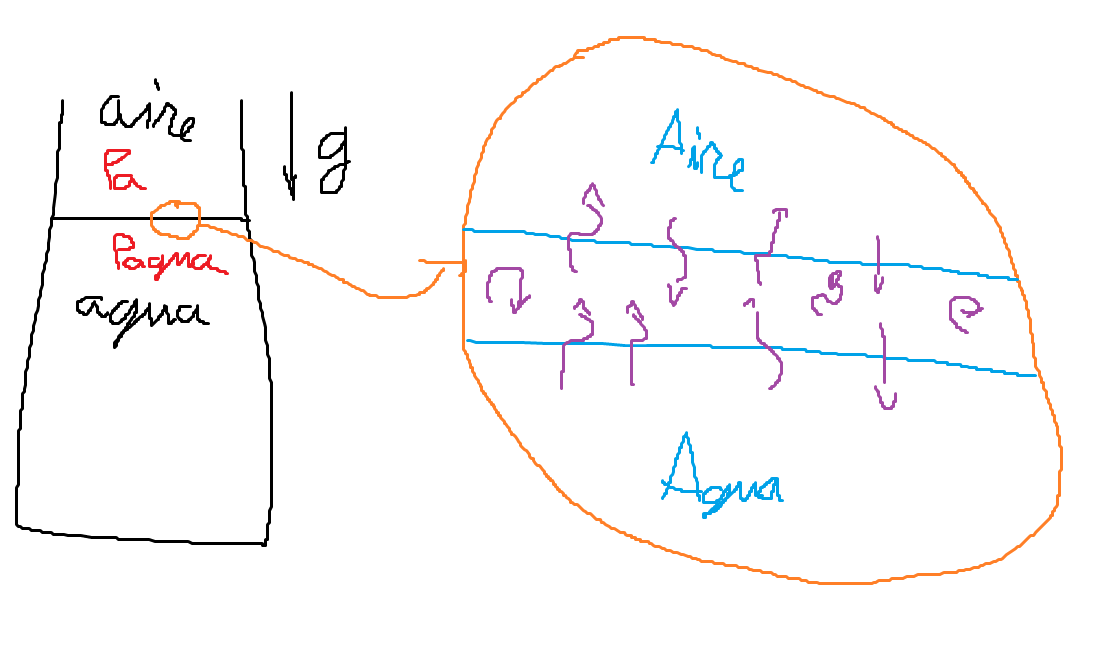
\includegraphics[width=0.5\linewidth]{imagenesTema1/vasoGrande}
		 %	\caption{Interfase Vaso grande.}
		 %	\label{fig:vasogrande}
		 %\end{figure}

		 \begin{figure}[H]
		 	\centering
		 		\begin{circuitikz}[scale=0.7]
		 			\tikzstyle{every node}=[font=\normalsize]
		 			\draw [short] (2.75,20.75) -- (2.75,17);
		 			\draw [short] (2.75,17) -- (5.25,17);
		 			\draw [short] (5.25,17) -- (5.25,20.75);
		 			\draw [color={rgb,255:red,0; green,128; blue,255}, short] (2.75,20) -- (5.25,20);
		 			\node [font=\normalsize] at (4,20.75) {$P_a$};
		 			\node [font=\normalsize, color={rgb,255:red,0; green,128; blue,255}] at (4,19.5) {$P_{agua}$};
		 			\draw [-latex] (2,21.25) -- (2,20.25)node[pos=0.5,left]{$\vec{g}$};
		 			\node [font=\normalsize] at (4,21.5) {Aire};
		 			\node [font=\normalsize, color={rgb,255:red,0; green,128; blue,255}] at (4,18.75) {Agua};
		 			\draw  (9.5,19) circle (2cm);
		 			\draw [short] (4.5,20) -- (9.25,21);
		 			\draw [short] (4.5,20) -- (8.5,17.25);
		 			\draw [ color={rgb,255:red,0; green,128; blue,255}, short] (7.5,19.5) -- (11.5,19.5);
		 			\draw [ color={rgb,255:red,0; green,128; blue,255}, short] (7.5,18.5) -- (11.5,18.5);
		 			\node [font=\normalsize] at (9.5,20.5) {Aire};
		 			\node [font=\normalsize] at (9.5,17.5) {Agua};
		 			\draw [ color={rgb,255:red,128; green,0; blue,255}, -latex] (8,18.25) -- (8.25,18.75);
		 			\draw [ color={rgb,255:red,128; green,0; blue,255}, -latex] (8,19.75) -- (8.5,19.25);
		 			\draw [ color={rgb,255:red,128; green,0; blue,255}, -latex] (9.25,19.25) -- (9.5,19.75);
		 			\draw [ color={rgb,255:red,128; green,0; blue,255}, -latex] (9.25,18.75) -- (9.5,18.25);
		 			\draw [ color={rgb,255:red,128; green,0; blue,255}, -latex] (10.75,19.25) -- (10.25,19.75);
		 			\draw [ color={rgb,255:red,128; green,0; blue,255}, -latex] (10.75,18.75) -- (10.5,18.25);
		 			\draw [ color={rgb,255:red,128; green,0; blue,255}, -latex] (10.25,19) -- (9.75,19);
		 			\draw [ color={rgb,255:red,128; green,0; blue,255}, -latex] (11.5,18.75) -- (11,19);
		 			\draw [ color={rgb,255:red,128; green,0; blue,255}, -latex] (7.5,19) -- (8,19.25);
		 		\end{circuitikz}
		 	
		 	\caption{Interfase Vaso grande.}
		 	\label{fig:vasogrande}
		 \end{figure}
		 

		\item Vaso pequeño: Existe efecto de la tensión superficial $\left(\sigma \left[
		\dfrac{N}{m}\right]\right)$ descrita mediante la ecuación de Laplace-Young. Solo aplica a fluidos inmiscibles. 

		\begin{figure}[H]
			\hspace{0.1\textwidth}
			\begin{minipage}{0.5\textwidth}
				%\centering
				%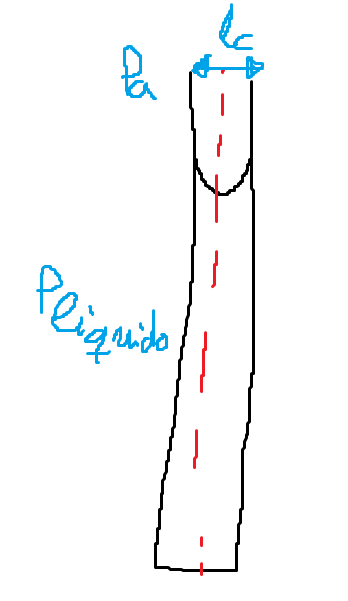
\includegraphics[width=0.2\linewidth]{imagenesTema1/vasoPeque}
				%\caption{Efecto tensión superficial Vaso pequeño}
				%\label{fig:vasopeque}
				
				\begin{figure}[H]
					\centering
					\begin{circuitikz}[scale=0.7]
						\tikzstyle{every node}=[font=\normalsize]
						\draw [short] (3.25,21) -- (3.25,15.75);
						\draw [short] (3.25,15.75) -- (4.25,15.75);
						\draw [short] (4.25,15.75) -- (4.25,21);
						\draw [ color={rgb,255:red,0; green,128; blue,255}, short] (3.25,20.5) .. controls (3.7,20.3) and (3.8,20.3) .. (4.25,20.5);
						\draw [ color={rgb,255:red,0; green,128; blue,255}, latex-latex] (3.25,21.5) -- (4.25,21.5)node[pos=0.5,above]{$l_c$};
						\node [font=\normalsize, color={rgb,255:red,0; green,128; blue,255}] at (3.75,18.25) {$P_{liq}$};
						\node [font=\normalsize, color={rgb,255:red,3; green,3; blue,3}] at (5,19) {$P_{a}$};
					\end{circuitikz}
					
					\caption{Efecto de la tensión superficial en un vaso pequeño}
					\label{fig:vasopeque}
				\end{figure}
			\end{minipage}
			\hspace{-0.05\textwidth}
			\begin{minipage}{0.5\textwidth}
				\[P_a - P_{liquido}=\sigma K\]
				\[K \ \text{expresión de la curvatura}\]
				\[K=\nabla_s \vec{n} = \left(\frac{1}{R_i}+\frac{1}{R_j}\right) \]
				\[R_i \ y \  R_j \ \text{son radios característicos}\]
			\end{minipage}
		\end{figure}

		\item Zona de efecto: La tensión superficial siempre presenta efectos, no obstante solo se aprecia en una región concreta.

		\[\rho g l_c \approx \sigma \Rightarrow l_c \approx \left(\frac{\sigma}{\rho g}\right)^{\frac{1}{2}}\]
		
		\begin{figure}[H]
			%\centering
			%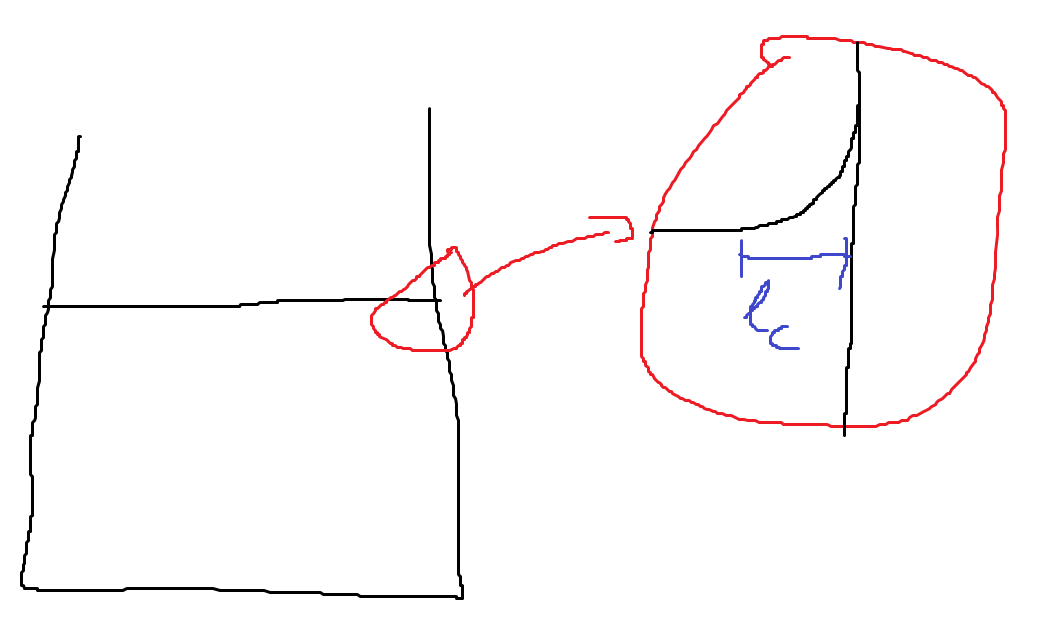
\includegraphics[width=0.4\linewidth]{imagenesTema1/zonaEfectos}
			%\caption{Zona de efecto.}
			%\label{fig:zonaefectos}
			
			\begin{figure}[H]
				\centering
					\begin{circuitikz}[scale=0.7]
						\tikzstyle{every node}=[font=\normalsize]
						\draw [short] (-1.75,21.5) -- (-1.75,17.75);
						\draw [short] (-1.75,17.75) -- (1,17.75);
						\draw [short] (1,17.75) -- (1,21.5);
						\draw [ color={rgb,255:red,0; green,128; blue,255}, short] (-1.75,20.75) -- (1,20.75);
						\draw [ color={rgb,255:red,255; green,0; blue,0} ] (1,20.75) circle (0.5cm);
						\draw [ color={rgb,255:red,255; green,0; blue,0} ] (4.75,20.75) circle (1.75cm);
						\draw [ color={rgb,255:red,255; green,0; blue,0}, short] (0.77,21.2) -- (4.25,22.425);
						\draw [ color={rgb,255:red,255; green,0; blue,0}, short] (0.77,20.3) -- (4.25,19.07);
						\draw [ color={rgb,255:red,0; green,128; blue,255}, short] (3,20.75) -- (5,20.75);
						\draw [ color={rgb,255:red,0; green,128; blue,255}, short] (5,20.75) .. controls (5.75,20.75) and (6,21) .. (6,22);
						\draw [ color={rgb,255:red,0; green,128; blue,255}, latex-latex] (5.25,20.5) -- (6,20.5)node[pos=0.5,below]{$l_c$};
						\draw [short] (6,22) -- (6,19.5);
					\end{circuitikz}
				\caption{Zona de efecto.}
				\label{fig:zonaefectos}
			\end{figure}
		\end{figure}
		
		\item Casos particulares
		\begin{enumerate}
			\item Chorro
			\begin{figure}[H]
				\begin{minipage}{0.5\textwidth}
				%\centering
				%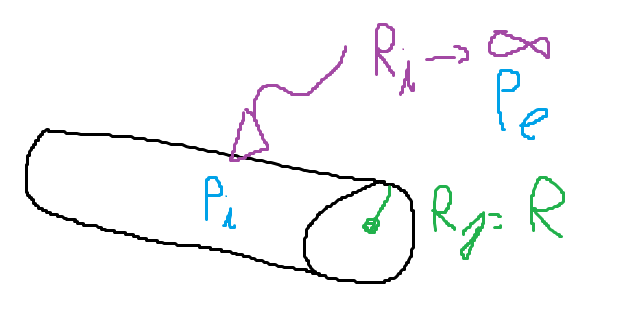
\includegraphics[width=0.7\linewidth]{imagenesTema1/chorro}
				%\caption{Chorro.}
				%\label{fig:chorro}
				
				\begin{figure}[H]
					\centering
						\begin{circuitikz}
							\tikzstyle{every node}=[font=\normalsize]
							\node [font=\normalsize, color={rgb,255:red,0; green,128; blue,255}] at (1.25,16.75) {$P_i$};
							\draw [short] (0.25,17.5) -- (3.25,17.5);
							\draw [short] (0.25,16) -- (3.25,16);
							\draw [ color={rgb,255:red,0; green,128; blue,0}, -latex] (3.25,16.75) -- (3.25,17.5)node[pos=1.2,right]{$R_j=R$};
							\draw  (3.25,16.75) ellipse (0.5cm and 0.75cm);
							\draw [short] (0.25,17.5) .. controls (-0.25,17.25) and (-0.25,16.25) .. (0.25,16);
							\node [font=\normalsize] at (1.25,15.5) {$P_e$};
							\draw [ color={rgb,255:red,128; green,0; blue,255}, -latex] (1.75,18.5) -- (1.75,17.5)node[pos=0,above]{$R_i$ $\Rightarrow$ $\infty$};
						\end{circuitikz}
					
					\caption{Chorro.}
					\label{fig:chorro}
				\end{figure}
				
			\end{minipage}%
			\begin{minipage}{0.5\textwidth}
			\[P_i - P_e =\sigma\left(\frac{1}{R_i}+\frac{1}{R_j}\right)=\frac{\sigma}{R}\]
			
			\end{minipage}
			\end{figure}
			
			
			\item Gota
			
			\begin{figure}[H]
				\begin{minipage}{0.5\textwidth}
				%\centering
				%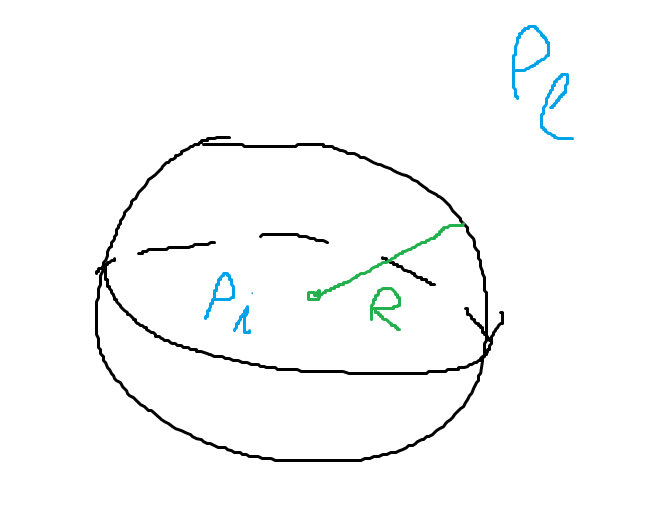
\includegraphics[width=0.7\linewidth]{imagenesTema1/gota}
				%\caption{Gota.}
				%\label{fig:gota}
				
				\begin{figure}[H]
					\centering
						\begin{circuitikz}
							\tikzstyle{every node}=[font=\normalsize]
							\draw  (2.25,17.5) circle (2cm);
							\draw [dashed] (0.25,17.5) .. controls (1,18.25) and (3.5,18.25) .. (4.25,17.5);
							\draw [short] (0.25,17.5) .. controls (1,16.75) and (3.5,16.75) .. (4.25,17.5);
							\draw [ color={rgb,255:red,0; green,128; blue,0}, -latex] (2.25,17.5) -- (3.5,19)node[pos=0.35,above]{R};
							\node [font=\normalsize, color={rgb,255:red,0; green,128; blue,255}] at (1.5,18.5) {$P_i$};
							\node [font=\normalsize] at (3.5,19.75) {$P_e$};
						\end{circuitikz}
					
					\caption{Gota.}
					\label{fig:gota}
				\end{figure}
				
				\end{minipage}%
				\begin{minipage}{0.5\textwidth}
				\[P_i - P_e =\sigma\left(\frac{1}{R_i}+\frac{1}{R_j}\right)=\frac{2\sigma}{R}\]
				
				\end{minipage}
				
			\end{figure}
			
			\item Pompa
			
			\begin{figure}[H]
				\begin{minipage}{0.5\textwidth}
				%\centering
				%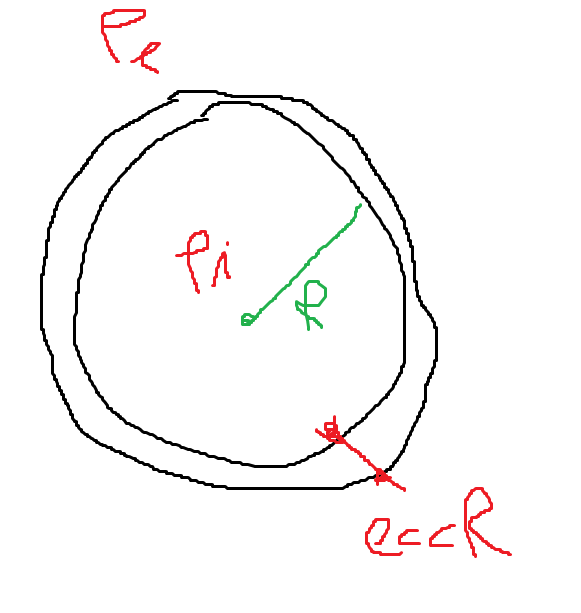
\includegraphics[width=0.7\linewidth]{imagenesTema1/pompa}
				%\caption{Pompa.}
				%\label{fig:pompa}
				
				\begin{figure}[H]
					\centering
						\begin{circuitikz}
							\tikzstyle{every node}=[font=\normalsize]
							\draw  (2.25,17.5) circle (2cm);
							\draw [dashed] (0.25,17.5) .. controls (1,18.25) and (3.5,18.25) .. (4.25,17.5);
							\draw [short] (0.25,17.5) .. controls (1,16.75) and (3.5,16.75) .. (4.25,17.5);
							\draw [ color={rgb,255:red,0; green,128; blue,0}, -latex] (2.25,17.5) -- (3.5,19)node[pos=0.35,above]{R};
							\node [font=\normalsize, color={rgb,255:red,0; green,128; blue,255}] at (1.5,18.5) {$P_i$};
							\node [font=\normalsize] at (3.5,19.75) {$P_e$};
							\draw  (2.25,17.5) circle (1.75cm);
							\draw [short] (0.5,17.5) .. controls (1,17) and (3.5,17) .. (4,17.5);
							\draw [dashed] (0.5,17.5) .. controls (1,18) and (3.5,18) .. (4,17.5);
							\draw [ color={rgb,255:red,255; green,0; blue,0}, short] (2.25,15.75) -- (2.25,15.5);
							\draw [ color={rgb,255:red,255; green,0; blue,0}, -latex] (2.25,15) -- (2.25,15.5)node[pos=0.5,left]{$e<\!<R$};
							\draw [ color={rgb,255:red,255; green,0; blue,0}, -latex] (2.25,16.25) -- (2.25,15.75);
						\end{circuitikz}
					
					\caption{Pompa.}
					\label{fig:pompa}
				\end{figure}
				
			\end{minipage}%
			\begin{minipage}{0.5\textwidth}
			\[P_i - P_m =\frac{2\sigma}{R}\]
			\[P_m - P_e =\frac{2\sigma}{R}\]
			\[P_i - P_e =\frac{4\sigma}{R}\]
			
			\end{minipage}
			\end{figure}
			
			\newpage
			
			\item Plano
			
			\begin{figure}[H]
			\begin{minipage}{0.5\textwidth}
				%\centering
				%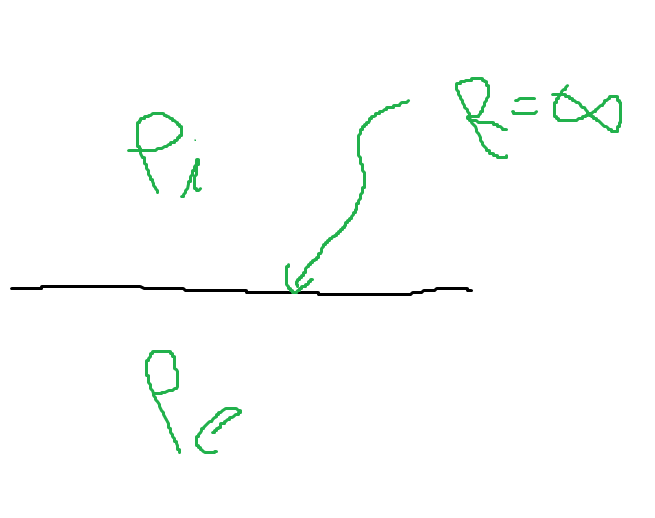
\includegraphics[width=0.7\linewidth]{imagenesTema1/plano}
				%\caption{Plano.}
				%\label{fig:plano}
				
				\begin{figure}[H]
					\centering
						\begin{circuitikz}
							\tikzstyle{every node}=[font=\normalsize]
							\draw [short] (-0.5,18) -- (3.5,18);
							\draw [ color={rgb,255:red,128; green,0; blue,255}, -latex] (2,19.75) -- (2,18)node[pos=0.5,right]{$R \Rightarrow \infty$};
							\node [font=\normalsize] at (0.5,18.5) {$P_i$};
							\node [font=\normalsize] at (0.5,17.5) {$P_e$};
						\end{circuitikz}
					
					\caption{Plano.}
					\label{fig:plano}
				\end{figure}
				
			\end{minipage}%
			\begin{minipage}{0.5\textwidth}
			\[P_i - P_e =\sigma\left(\frac{1}{R_i}+\frac{1}{R_j}\right)=0\Rightarrow P_i = P_e\]
			
			\end{minipage}
			\end{figure}
			
		\end{enumerate}
	\end{itemize}
\end{enumerate}

\section{Mojabilidad.}
\begin{itemize}
	\item Un líquido no moja a un sólido si $\theta_c \gtrsim \ang{150} $. Sólido hidrofóbico.
	\item Un líquido moja a un sólido si $\theta_c  \lesssim \ang{45}$. Sólido hidrofílico totalmente.
\end{itemize}
\begin{figure}[H]
	%\centering
	%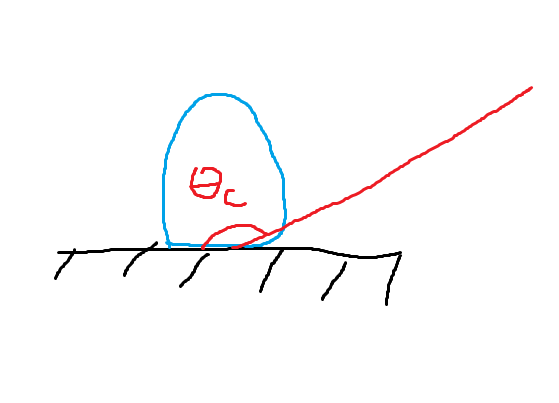
\includegraphics[width=0.7\linewidth]{imagenesTema1/mojabilidad}
	%\caption{Mojabilidad.}
	%\label{fig:mojabilidad}
	
	\begin{figure}[H]
		\centering
			\begin{circuitikz}
				\tikzstyle{every node}=[font=\normalsize]
				\draw [short] (-0.5,18.25) -- (3.5,18.25);
				\draw [short] (-0.25,18.25) -- (-0.5,18);
				\draw [short] (0.25,18.25) -- (0,18);
				\draw [short] (0.75,18.25) -- (0.5,18);
				\draw [short] (1.25,18.25) -- (1,18);
				\draw [short] (1.75,18.25) -- (1.5,18);
				\draw [short] (2.25,18.25) -- (2,18);
				\draw [short] (2.75,18.25) -- (2.5,18);
				\draw [short] (3.25,18.25) -- (3,18);
				\draw [ color={rgb,255:red,255; green,0; blue,0}, short] (1.75,18.25) -- (3.5,20);
				\draw [ color={rgb,255:red,255; green,0; blue,0}, short] (2.25,18.75) .. controls (1.75,19) and (1.25,18.75) .. (1,18.25)node[pos=0.5,above]{$\theta_c$};
				\draw [ color={rgb,255:red,0; green,128; blue,255}, short] (2.5,19) .. controls (2.75,19.75) and (2.25,20) .. (1.5,20);
				\draw [ color={rgb,255:red,0; green,128; blue,255}, short] (1.5,20) .. controls (0.5,20) and (-0.5,18.25) .. (0.5,18.25);
				\draw [ color={rgb,255:red,0; green,128; blue,255}, short] (0.5,18.25) .. controls (1,18.25) and (1.25,18.25) .. (1.75,18.25);
				\draw [ color={rgb,255:red,0; green,128; blue,255}, short] (1.75,18.25) -- (2.5,19);
			\end{circuitikz}
		\caption{Mojabilidad.}
		\label{fig:mojabilidad}
	\end{figure}
	
\end{figure}
